\chapter{poglavlje}{Arhitektura}
U ovom se poglavlju opisuje arhitektura predloženog (kasnije i implementiranog) sustava. Opisuje se način na koji je lokalna mreža usmjerena
kroz pristupnu točku, gdje se i kako prikuplja mrežni promet te kako se prikupljeni podatci pohranjuju, vizualiziraju te u konačnici kako se s tim podatcima 
rukuje kako bi se postigla automatska detekcija. Naglasak je na odlukama o dizajnu i njihovim opravdanjima, dok se konkretna implementacija obrađuje kasnije.

\section{Pregled sustava}
Sustav je zamišljen da pretvori uređaj s mrežnim mogućnostima u jedinstvenu točku kroz koju prolazi sav promet lokalne
mreže, čime se ostvaruje potpuna vidljivost komunikacije između lokalnih uređaja i vanjskih odredišta. Taj uređaj
istovremeno obavlja funkciju usmjernika (eng.\ \emph{gateway}), pristupne točke, mrežnog senzora i vatrozida.

Slika \ref{fig:tok-podataka} prikazuje tok podataka kroz sustav. Sav mrežni promet prolazi kroz pristupnu točku gdje ga Zeek pasivno analizira i pohranjuje 
u obliku strukturiranih JSON zapisa u dijeljeni direktorij.
Iz tog se direktorija podatci paralelno "šalju" u dva odvojena podsustava za pohranu. Prvi sustav čine vremenski orijentirana baza InfluxDB posredstvom 
podatkovnog agregatora Telegrafa. Drugi sustav čine dokumentno orijentiranu bazu Elasticsearch posredstvom agenta zvanog Filebeat. 
Oba podsustava kao zajedničko vizualizacijsko sučelje koriste Grafanu. Usporedno postojanje dvaju podsustava ne predstavlja produkcijsku konfiguraciju, već
služi za njihovu usporedbu opisanu u kasnijim poglavljima. U stvarnoj bi se primjeni odabrao jedan od njih ovisno o potrebama i mogućnostima.

\begin{figure}[ht]
  \centering
  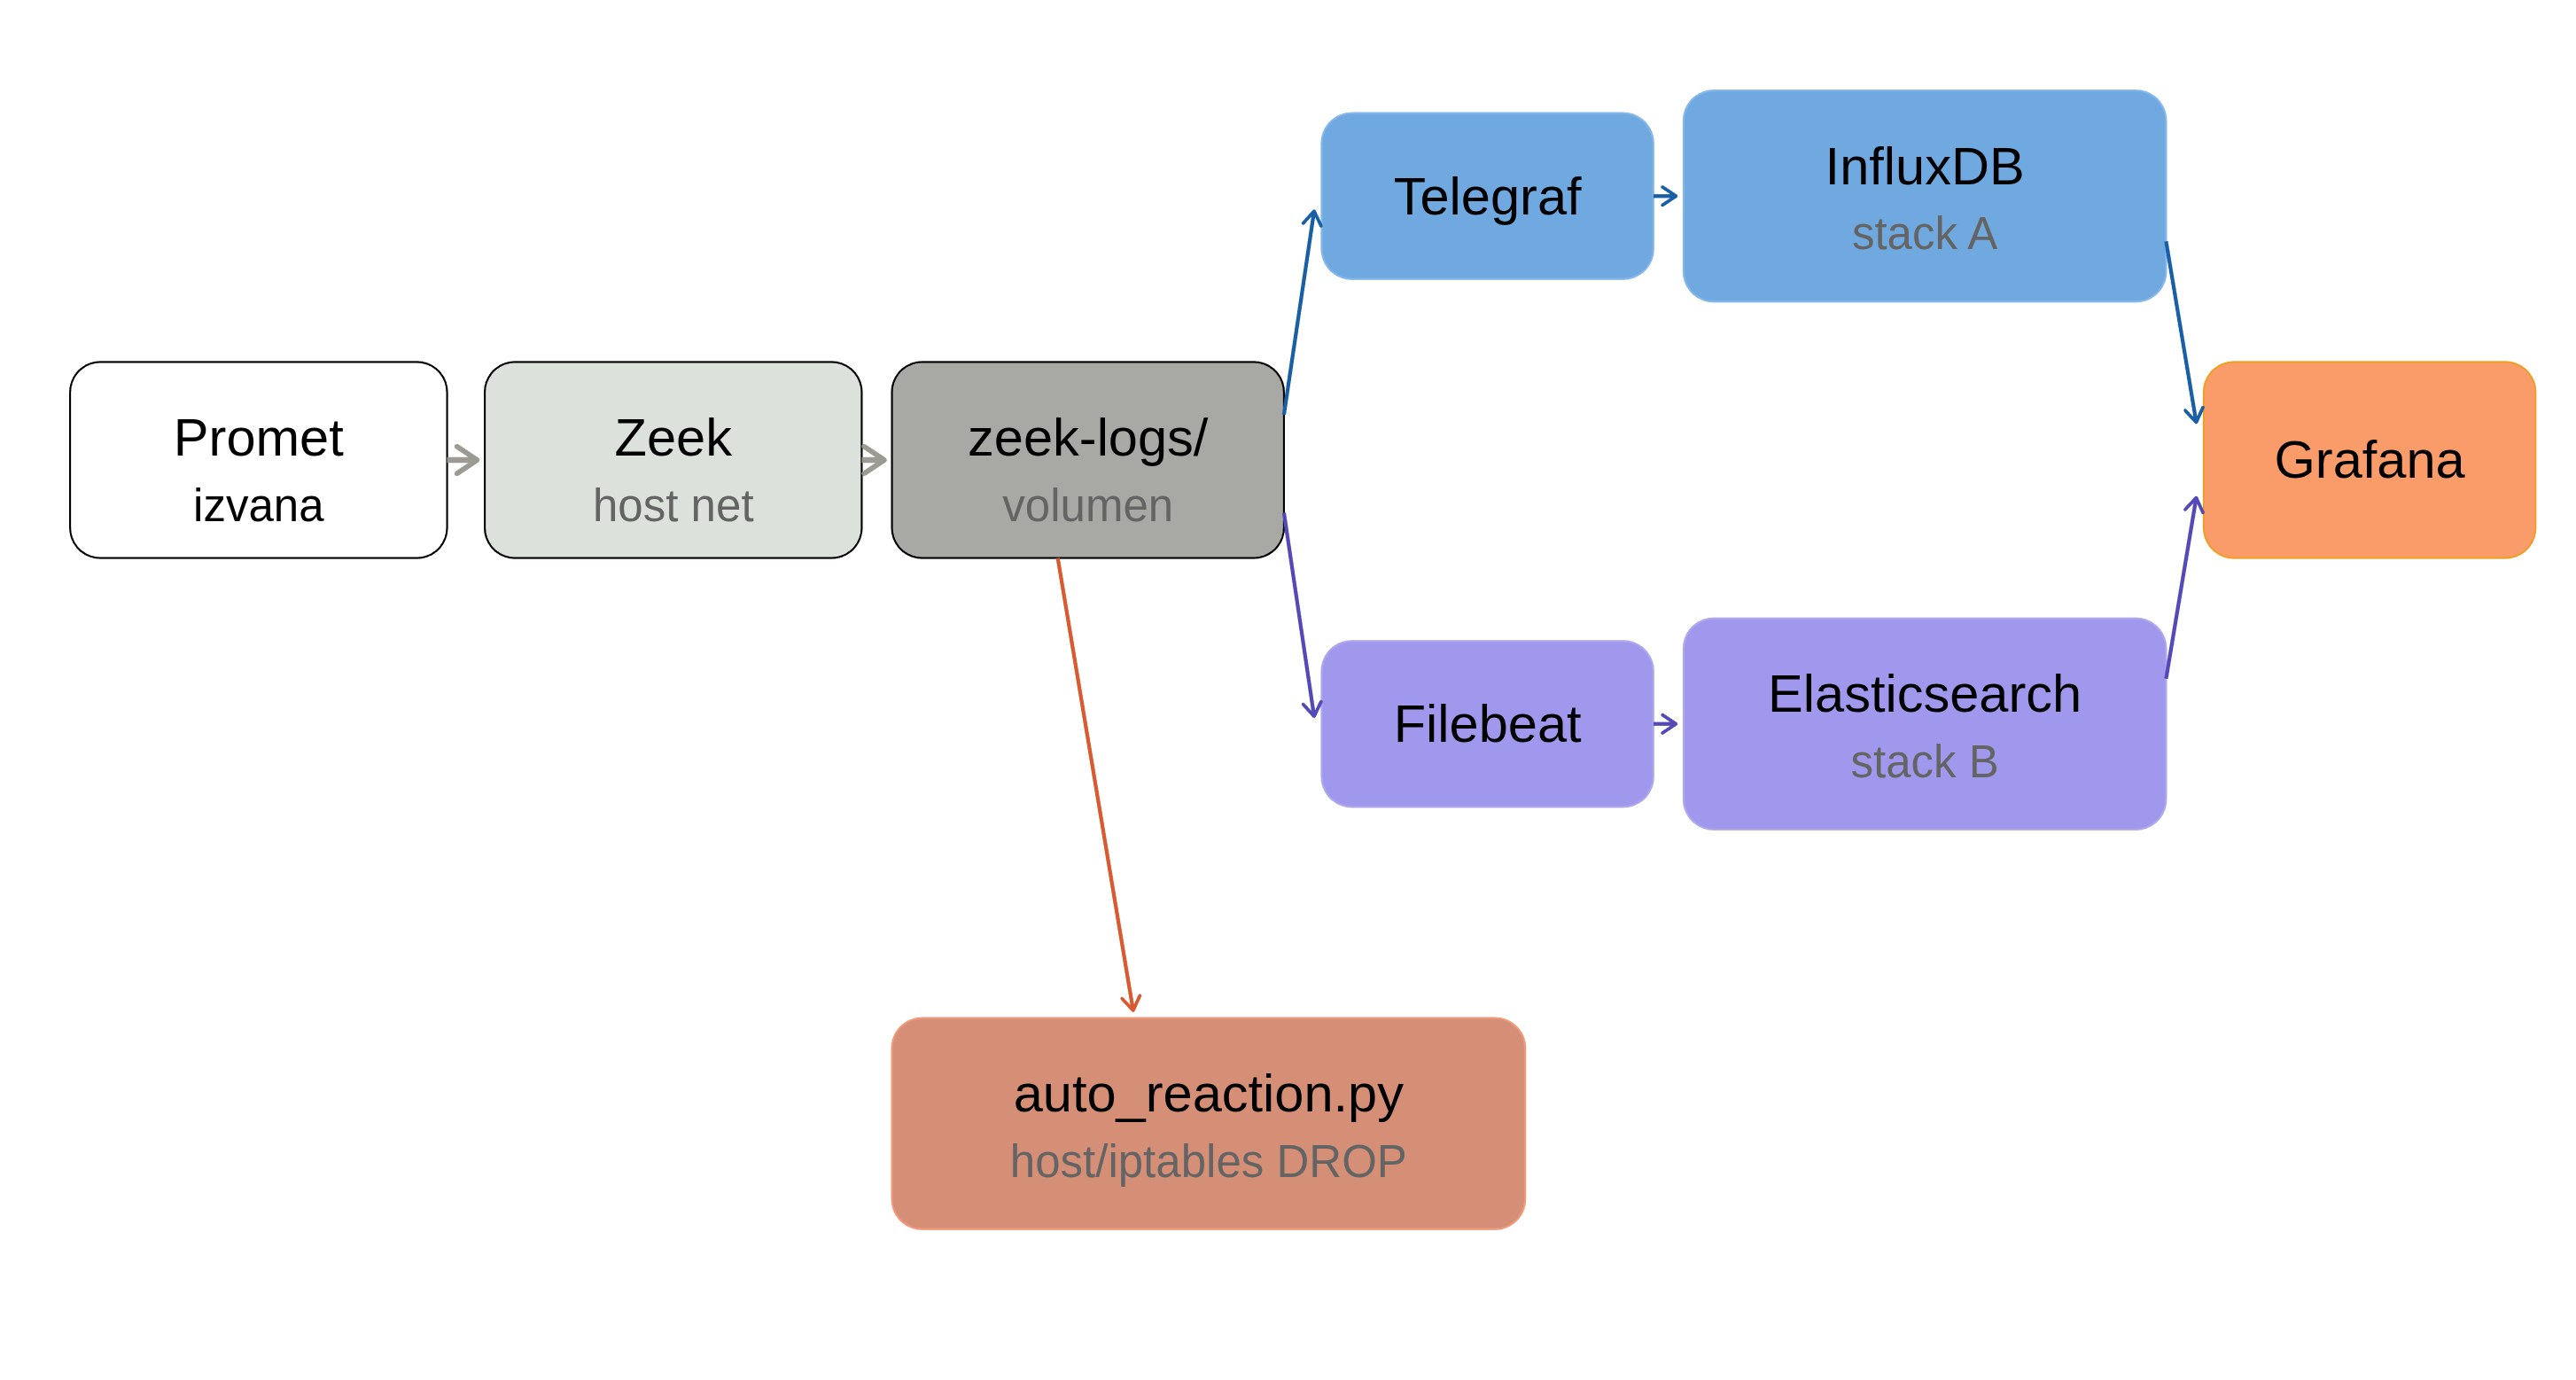
\includegraphics[width=0.95\textwidth]{slike/tok_podataka_dual_stack_custom.png}
  \caption{Prikaz toka podataka kroz sustav}
  \label{fig:tok-podataka}
\end{figure}

Svi navedeni servisi izvode se u Docker kontejnerima, čime se postiže ponovljivost i prenosivost okruženja te jednostavnost pri postavljanju \cite{docker_docs}. 
Jedina je iznimka skripta za automatsku reakciju, koja se izvodi izravno na domaćinu iz kasnije objašnjenih razloga.

\section{Mrežni sloj}
Mrežna topologija sustava prikazana je na slici \ref{fig:topologija}. 

\begin{figure}[h]
  \centering
  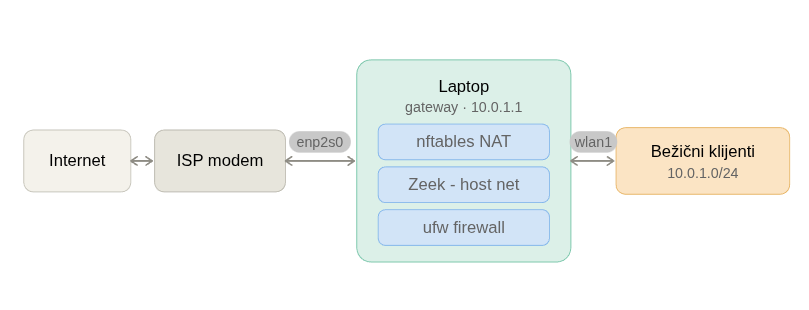
\includegraphics[width=0.95\textwidth]{slike/mrezna_topologija_custom.png}
  \caption{Mrežna topologija. Prijenosno računalo objedinjuje uloge rutera,
           pristupne točke, senzora i vatrozida}
  \label{fig:topologija}
\end{figure}

\section{Nadzorni sloj}

\section{Tok podataka i pohrana}

\section{Prepoznavanje i automatska reakcija}
